\section{Pipeline Hazards}
\sloppy
Vi sono situazioni, denominate \textit{hazards}, nelle quali viene impedito alla prossima istruzione nel flusso di istruzioni della pipeline di venire eseguita nel ciclo di clock designato.

Distinguiamo: hazards \textbf{strutturali}, che sorgono a causa di conflitto tra risorse hardware, ovvero quando l'hardware non riesce a supportare tutte le possibili combinazioni di istruzioni simultaneamente in esecuzioni sovrapposte; hazards \textbf{sui dati}, che sorgono quando un'istruzione dipende dal risultato di un'istruzione precedente; hazards \textbf{di controllo}, che sorgono in casi di istruzioni di branch e in generale di istruzioni che modificano il PC. Spesso, per risolvere un hazard è necessario fermare la pipeline, ovvero forzare una \textit{stall}. Nello situazione in cui un'istruzione viene fermata, tutte le istruzioni successive a questa vengono fermate, mentre quelle precedenti continuano il loro flusso di attraversamento della pipe. Gli hazards strutturali sono poco frequenti in quanto riguardano unità funzionali hardware (come l'unità di divisione a virgola mobile) non utilizzate frequentemente, perchè sia i programmatori che i compilatori sono a conoscenza di questo tipo di hazards. Ci concentreremo principalmente sui data hazards e sui control hazards. 

\subsection{Hazards sui dati}
La sovrapposizione di istruzioni introdotta dalla pipeline implica un cambiamento dell'ordine di accessi in lettura/scrittura agli operandi rispetto al modello sequenziale di Von Neumann. Un primo passo risolutivo è già stato presentato: quando si cerca di leggere o scrivere da uno stesso registro contemporaneamente, molte architetture prevedono che la scrittura avvenga nella prima metà del ciclo di clock mentre la lettura nella seconda metà. Questo risolve l'hazard quando la scrittura del registro avviene durante lo stesso ciclo di clock della lettura. 

\noindent In linea di massima, il dato prodotto dall'istruzione da cui dipendono le successive è già pronto durante la fase di execute, quindi basterebbe semplicemente propagare il dato appena è possibile alle unità a cui serve prima che sia disponibile per la lettura dal file register. Ci occuperemo per semplicità solo del caso di propagazione in una fase EX, che può essere la propagazione di un risultato di una operazione ALU o il calcolo di un indirizzo effettivo. Questo significa che quando un'istruzione prova ad usare un registro nella sua fase EX che un'istruzione precedente deve ancora scrivere in fase di WB, può servirsi del valore anticipatamente come input controllato alla ALU.

\noindent Un caso in cui il forwarding non può risolvere l'hazard è quando un'istruzione prova a leggere un registro immediatamente dopo un'istruzione di \textit{load} dalla memoria. Il dato risulterebbe ancora in fase di recupero dalla memoria, quindi è necessaria un'unità funzionale che stalli la pipeline. In generale, il compialtore, che è a conoscenza della struttura del processore, in casi di hazard detection di questo tipo si preoccupa di anticipare delle istruzioni indipendenti utilizzando la proprietà commutativa e associativa. Lo stallo è inevitabile quando non è possibile inserire dopo l'istruzione di accesso in memoria un blocco di istruzioni indipendenti. \uppercase{è} possibile tuttavia un approccio, denominato \textbf{internal forwarding}, che permette di ibernare temporaneamente le istruzioni bloccate, e non stallare la pipeline. Bloccando istruzioni e caricandone altre, tuttavia può accadere che più istruzioni cerchino di operare sullo stesso registro, quindi occorre utilizzare una tecnica di indirizzamento indiretto che permette ai registri fisici del processore (\textit{forwarding registers}) di puntare a dei registri in memoria che contengono valori precedenti assunti dal registro. Le istruzioni vengono ibernate in un'apposita area della memoria, la \textit{ibernation table}. 

\subsection{Hazards di controllo} \label{subsec:control_hazards}
Quando sopraggiunge un istruzione di salto, riusciamo a captare che è così solo nella fase di esecuzione dell'istruzione, mentre la pipe ha continuato a caricare le istruzioni in modo sequenziale, che si troveranno rispettivamente nella fase di IF e ID e non avranno quindi ancora modificato lo stato del processore e della memoria. Nel caso in cui il salto non deve essere eseguito, allora la pipe continuerà a funzionare normalmente, mentre se il salto deve essere eseguito, le istruzioni caricate dovranno essere eliminate dalla pipe (\textit{pipe flush}) e dovrà essere caricata l'istruzione a cui punta il salto e le successive. Il ritardo che segue quest'ultimo caso è detto \textit{branch penalty}. L'obiettivo è quello di confinare la gestione dei salti nelle fasi IF e ID, perchè in quelle fasi le istruzioni non hanno ancora modificato lo stato del processore e della memoria, e quindi la rete di controllo hardware deve riguardare solo queste due fasi.
In generale, il problema è risolvibile fondamentalmente mediante due approcci: l'approccio conservativo e l'approccio ottimistico (\textit{branch prediction}).
Nel caso dell'\textbf{approccio conservativo}, quando il processore interpreta, durante la fase ID, un'istruzione come istruzione di salto, ferma la pipe e disabilita la propagazione dell'istruzione che si trova erroneamente nella fase IF, determina l'istruzione a cui saltare in fase EX e la preleva. Si torna insomma al modello sequenziale di Von Neumann. Il conto è salato se consideriamo che le istruzioni di salto costituiscono il 25\% di un programma, e infatti ne consegue un notevole spreco delle risorse di parallelismo fornite dalla pipe. Questo approccio è \textit{leggermente} migliorabile attraverso l'hardware, anticipando la decisione inerente al salto alla fase di ID, in base alla condizione di salto. Ad esempio l'istruzione \lstinline|JNZ <LABEL>| controlla se il flag Z del SR è alto, e in tal caso non occorre saltare e quindi l'istruzione che si è prelevata nel frattempo è giusta. Molti ritardi possono essere  evitati dal programmatore o dal compilatore: il programmatore può contribuire al buon funzionamento del sistema, scrivendo le istruzioni in un ordine tale da minimizzare le probabilità di stallo della pipe. Nel caso di un costrutto if-then-else, ad esempio, conviene inserire nel ramo then l'alternativa più probabile. Il compilatore, da parte sua, può operare vari accorgimenti; ad esempio, siccome un ciclo for è sempre tradotto in un if-then-else, esso deve inserire l'alternativa più probabile nel ramo then.
In fase di compilazione è possibile evitare l'approccio conservativo. Se immediatamente prima del salto c'è un'istruzione con operandi da cui non dipende l'esito della scelta di saltare o meno, è possibile in fase di compilazione inserire l'istruzione indipendente dopo il branch, in modo da sfruttare lo slot di tempo in cui l'istruzione viene caricata ed entra nella pipe, e quindi non c'è bisogno di pipe flush. Qualora non sia possibile invertire una istruzione if con quella che la precede, il compilatore potrebbe decidere di mettere subito dopo la if una \textbf{nop}, istruzione che non ha alcun effetto e quindi non è mai errato inserirla nella pipe. In questo modo si può operare senza considerare alcun tipo di approccio. Possiamo aggiungere che se stiamo considerando un'istruzione di salto in un processore CISC con una condizione di salto elaborata, allora il numero di nop che bisogna inserire a seguito dell'istruzione di salto risulta essere superiore a 1, in quanto ricordiamo che la pipe per i CISC è più lunga e la valutazione della condizione coinvolge più fasi oltre le prime due, di caricamento e decodifica.
Una soluzione meno conservativa a quella appena presentata è di utilizzare la \textbf{branch-prediction} $\rightarrow$ approccio ottimistico.

\noindent La branch prediction è una tecnica che cerca di prevedere a quale ramo un' istruzione di salto condizionato possa saltare. Consideriamo il classico esempio:
\begin{lstlisting}[language=C]
for (int i = 0; i < N; i++){
    for (int j = 0; j < N; j++){
        op...
    }
}
\end{lstlisting}

Il controllo prevede l'esecuzione del ramo else una sola volta (guardando il for interno) ogni N passi.
I modi per prevedere il branch possono essere vari, e possono essere descritti mediante degli appositi automi a stati finiti. Un primo approccio molto basilare è quello di andare a cambiare il branch da caricare successivamente ad ogni errore di decisione e quindi eseguire le operazioni descritte dall'automa [\ref{img:automa-semplice}].

\begin{figure}[ht]
    \centering
    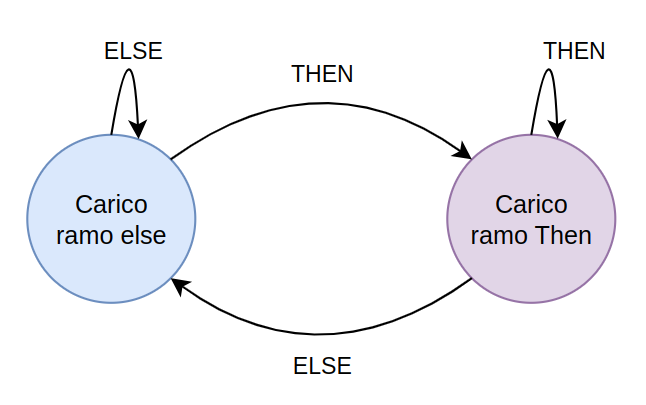
\includegraphics[width=.5\textwidth]{fig/chapter_1/automa-semplice.png}
    \caption{Automa della branch prediction base}\label{img:automa-semplice}
\end{figure}

Questa soluzione non è ottima poichè per quel singolo errore che avviene ad ogni N interazioni la pipeline dovrà assorbire 2 penalties. Per evitare tale condizione, e quindi rendere la persistenza più forte, consideriamo un automa a 4 stati che permette di rendere la condizione di "cambio del branch" più solida, poichè solo in caso di due errori successivi, allora cambio l'indirizzo di salto effettivo. L'automa a cui facciamo riferimento è [\ref{img:automa-complesso}].

\begin{figure}[ht]
    \centering
    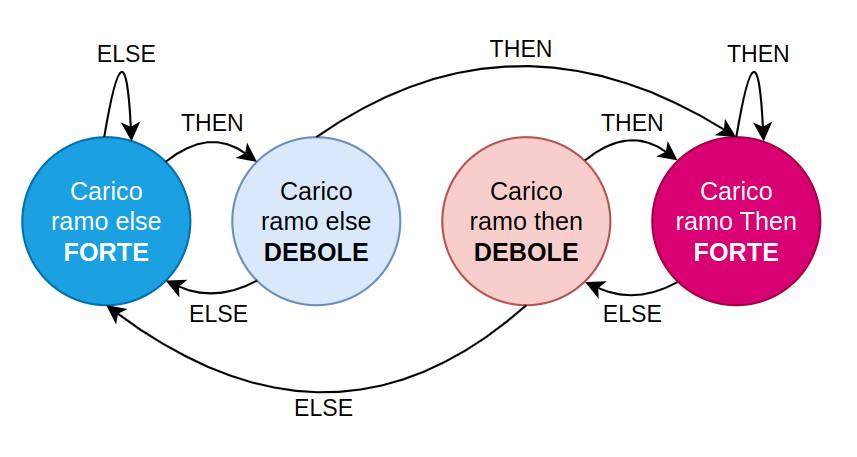
\includegraphics[width=.5\textwidth]{fig/chapter_1/automa-complesso.png}
    \caption{Automa della branch prediction avanzato}\label{img:automa-complesso}
\end{figure}

\noindent Per implementare la predizione a livello hardware, il processore utilizza una \textbf{tabella di predizione} dei salti. Una possibile struttura prevede i campi (Indirizzo dell'istruzione di salto, indirizzo di destinazione, 2 bit per codificare lo stato).

\noindent La tabella viene aggiornata in parallelo durante la fase di Execute (EX), ovvero nel momento in cui il processore verifica se la predizione è corretta. Se c'è stato un errore, si aggiorna lo stato dell'automa (e la corrispondente voce nella tabella). Tale struttura è memorizzata in un apposita area di memoria, detta \textbf{Branch History Table} (BHT).

Con l'introduzione del sistema a pipeline e del meccanismo dell'\textbf{internal forwarding}, che altera la sequenzialità delle istruzioni eseguite dal processore, nasce il problema della \textbf{gestione delle interruzioni}. 
Infatti può capitare che alcune istruzioni siano completate in un ordine diverso da quello in cui sono state avviate. In tal caso è possibile che si generino delle \textit{interruzioni non esatte}, cioè situazioni in cui un' istruzione provoca un' eccezione prima che tutte quelle che la precedono siano completate. Ovviamente, per la corretta gestione delle eccezioni stesse, l'obiettivo che ci si pone è quello di creare un sistema che sia in grado di arrestare opportunamente la pipe in modo da completare le istruzioni che precedono quella che ha generato l'interruzione senza avviare quelle che seguono, così da ottenere un comportamento che rispetti quello descritto dal modello di Von Neumann che viene definito di \textit{gestione precisa} delle interruzioni.
Le \textbf{interruzioni esterne} sono più facili da gestire: infatti la interrupt service routine relativa all'interruzione sopraggiunta verrà inserita nella pipeline come una normale istruzione, dopo che tutte le istruzioni precedenti verranno correttamente terminate, comprese quelle ibernate. 
Più critico è il caso delle \textbf{interruzioni interne}. Infatti questo genere di interruzioni possono essere causate da diverse istruzioni contemporaneamente all'interno della pipe in diversi stages. Non è dunque garantito il comportamento sequenziale di Von Neumann. Un esempio abbastanza lampante di conflitto è il caso in cui nella stessa pipe un'istruzione cerca di effettuare un accesso illegale in memoria (eccezione scatenata nella fase MEM) mentre un'altra istruzione, successiva, tenta una divisione per zero (eccezione scatenata nella fase ID).

\noindent Alcuni processori rinunciano del tutto ad avere interruzioni precise. In questo caso è compito del software assicurare che nella stessa pipeline non ci siano istruzioni le cui possibili eccezioni possano causare questo tipo di conflitto. Considerando il tasso di istruzioni che generano eccezione in un generico codice, questa soluzione può essere più o meno accettabile. Altri processori invece riescono a ricostruire interruzioni precise, utilizzando tecniche di tipo conservativo o ottimistico. 
Nelle tecniche di tipo \textbf{conservativo}, il processore fa procedere nella pipe un'istruzione finché è sicuro che non possa essere fonte di interruzione, e solo a questo punto ne avvia un'altra. Il parallelismo intrinseco della pipe è dunque limitato, a vantaggio della gestione precisa delle eccezioni. 

\noindent Nel caso di tecniche di tipo \textbf{ottimistico}, vengono inserite comunque istruzioni nella pipeline indipendentemente dalla possibilità di generare o meno eccezioni. Se emergono conflitti il sistema deve essere in grado di effettuare un \textit{rollback}, e quindi è necessaria un'immagine dello stato del sistema.  
Il rollback può essere effettuato mediante due tecniche:

\begin{itemize}
    \item \textbf{Check point}: Vengono effettuate periodici snapshot dello stato dei registri del processore, compreso il PC, conservate in una opportuna area di memoria. Nel momento in cui si verifica un'eccezione, vengono ricopiati i valori memorizzati nei registri del processore e si riprende l'esecuzione \textit{sequenziale} del programma, quindi un'istruzione per volta, a partire dall'ultimo valore di PC riportato nello snapshot. Occorre in questo caso scegliere con attenzione la frequenza di cattura dello snapshot. 
    \item \textbf{History Buffer}: Ogni istruzione eseguita viene memorizzata in un'area di memoria insieme ai valori dei propri operandi. Ogni istruzione memorizzata può essere cancelalta dal buffer solo quando tutte quelle che la precedono si sono concluse senza generare interruzione. \uppercase{è} possibile definire in questo modo una sequenza di operazioni UNDO da effettuare nel caso un'istruzione ibernata precedentemente causi un'eccezione. Questa tecnica è anche utile per garantire la gestione precisa delle interruzioni, facendo in modo che un'eccezione non venga gestita se prima non sono terminate correttamente (quindi senza causare eccezioni) le istruzioni ibernate.
\end{itemize}

